\documentclass[10pt,aspectratio=169,dvipsnames]{beamer}
\usetheme[]{Berlin}

\setbeamertemplate{footline}{
  \usebeamercolor[fg]{framesource}%
  \usebeamerfont{page number in head}%
  \hspace{0.2cm}
  \small \insertframenumber
  \vspace{0.2cm}
  \doclicenseIcon
  \hfill
  
\includegraphics[height=0.8cm]{logos/tub_logo.pdf}
  \hspace{0.2cm}
}

\setbeamercovered{transparent}

\setbeamertemplate{footline}[
 myframe number]

% PACKAGES
\usepackage[absolute,overlay]{textpos}
\usepackage[utf8]{inputenc}
\usepackage[official]{eurosym}
\usepackage{booktabs,multicol,multirow,tabularx,array}
\usepackage{subcaption}
\usepackage{parskip}
\usepackage{bm}
\usepackage{tikz}
\usepackage{adjustbox}
\usepackage[super]{nth}
\usepackage[version=4]{mhchem}
\usepackage{siunitx}

\sisetup{
  detect-all = true
}


\usepackage[
    type={CC},
    modifier={by},
    version={4.0},
]{doclicense}

% HYPERREFERENCES
\usepackage{hyperref}
\hypersetup{
	colorlinks=true,
	citecolor=tub-blue,
	linkcolor=tub-blue,
	urlcolor=tub-blue
}

\usepackage[sfdefault]{roboto}
\usepackage[normalem]{ulem}

% \usepackage[backend=biber,style=numeric-comp]{biblatex}
% \addbibresource{references.bib}

\newcolumntype{R}[1]{>{\raggedleft\arraybackslash}p{#1}}


% GRAPHICS	
\graphicspath{
    {graphics/},
    {figures/},
  }
\DeclareGraphicsExtensions{.pdf,.jpeg,.png,.jpg}

% FORMATTING
\setlength{\parskip}{6pt}
\linespread{1.1}
\newcommand{\seprule}{\par\noindent\textcolor{black!25}{\rule{\textwidth}{0.4pt}}}

% SOURCES
\setbeamercolor{framesource}{fg=gray}
\setbeamerfont{framesource}{size=\tiny}
\newcommand{\source}[1]{\begin{textblock*}{10cm}(3.6cm,8.25cm)
    \begin{beamercolorbox}[ht=0.5cm,right]{framesource}
        \usebeamerfont{framesource}\usebeamercolor[fg]{framesource} Source: {#1}
    \end{beamercolorbox}
\end{textblock*}}

% REFERENCES
% \usepackage[style=nature, doi=true, maxcitenames=3]{biblatex}
% \bibliography{bibliography}
% \renewcommand*{\bibfont}{\footnotesize}

% COLOR TEXT
\newcommand{\bl}[1]{\textcolor{tub-blue}{#1}}
\newcommand{\gr}[1]{\textcolor{tub-green}{#1}}
\newcommand{\rd}[1]{\textcolor{tub-red}{#1}}
\newcommand{\yl}[1]{\textcolor{tub-yellow}{#1}}
% \newcommand{\org}[1]{\textcolor{tub-orange}{#1}}
\newcommand{\cb}[1]{\colorbox{gray!20}{#1}}

\usepackage{array}% https://ctan.org/pkg/array
\makeatletter
\g@addto@macro{\endtabular}{\rowfont{}}% Clear row font
\makeatother
\newcommand{\rowfonttype}{}% Current row font
\newcommand{\rowfont}[1]{% Set current row font
   \gdef\rowfonttype{#1}#1%
}
\newcolumntype{L}{>{\rowfonttype}l}

\usepackage[most]{tcolorbox}
\tcbuselibrary{listingsutf8}

% Custom commands
\usepackage{caption}
\renewcommand{\figurename}{} % Removes the "Figure" text
\captionsetup[figure]{labelformat=empty, labelsep=none} % Removes numbering and colon


% FONT
%\usepackage{utopia}

% REFERENCES
%\usepackage[backend=biber,style=authoryear-comp]{biblatex}
%\bibliography{references.bib}

% TITLE PAGE
\title{
  \textbf{Exchange: dena // RESILIENT} \\
}
\vspace*{-.5cm}

% \author{STRIse}
\institute[Technische Universität Berlin] % (optional, but mostly needed)
{ 
  \normalsize
  \alert{Project overview} \\ 
  \footnotesize
  \url{https://resilient-project.github.io/} \\
  Digital Transformation in Energy Systems \\
  Technische Universität Berlin \\

  \vspace{0.3cm}

  06. November 2025
}

\date{}

\subject{IN4climate --- Kickoff Sprint CO2 Infrastruktur}

\titlegraphic{%
\vspace{-1cm}

\includegraphics[height=1cm,clip=true]{logos/cetp_logo.png}
\hspace{0.5cm}
\includegraphics[height=1cm,clip=true]{logos/ensys_short_logo.pdf}
\hspace{0.5cm}
\includegraphics[trim=0 0cm 0 0cm,height=1cm,clip=true]{logos/tub_logo.pdf}
\hspace{0.5cm}
\includegraphics[trim=0.2cm 0.6cm 0.6cm 0.2cm,height=1.1cm,clip=true]{logos/bmwe_en_logo.png}
}

\begin{document}

\addtocounter{framenumber}{-1}
{
  \setbeamertemplate{footline}{
    \usebeamercolor[fg]{framesource}%
    \usebeamerfont{page number in head}%
    \begin{center}
      \Large
      \doclicenseIcon
      \vspace{0.4cm}
    \end{center}
  } 
  \maketitle
}

\section{RESILIENT}
\begin{frame}{RESILIENT project partners}
  \centering
  
\includegraphics[width=0.85\textwidth]{other/resilient_partners}
  
  \footnotesize
  Funded through the \alert{CETPartnership 2022} call and by the \alert{German Federal Ministry for Economic Affairs and Energy (BMWE)} for the German project partners.

  \source{\url{https://resilient-project.github.io/}}
\end{frame}

\begin{frame}{Project overview}
  \footnotesize
  \begin{columns}
    \begin{column}{0.75\textwidth}
      \begin{itemize}
      \item \alert{Problem description}: The world is in a phase of \alert{uncertainty} and \alert{transformation} (geopolitics, energy transition, climate change); scenarios with single deterministic solutions are no longer sufficient.
      \item \alert{Project goal}: Development and demonstration of tools for resilient planning of the energy transition for industry, e-fuels, and networks.
      \item Builds on the already established, open-source, and globally used multi-vector energy system model \alert{Python for Power System Analysis (PyPSA)}.
      \item \alert{Methodological focus}: Optimisation under uncertainty (stochastic and robust), decomposition methods, and heuristics for resilience.
      \item \alert{Case studies}: \alert{Industrial transition in North Rhine-Westphalia}, grid planning in Baden-Württemberg, e-fuels in Scandinavia, and climate extreme events in France.
      \end{itemize}
    \end{column}
    \begin{column}{0.25\textwidth}
      
\includegraphics[width=1\textwidth]{logos/logo-secondary-light.png}
    \end{column}
  \end{columns}
\end{frame}

\begin{frame}{Working packages}
  \centering
  
\includegraphics[width=0.8\textwidth]{other/resilient_project_structure}
  \source{\url{https://resilient-project.github.io/}}
\end{frame}

% \begin{frame}{Selection of planned model developments}
%   \footnotesize
%   \begin{columns}[T] % align columns
%     \begin{column}{.5\textwidth}
%         \begin{minipage}[t][.45\textheight]{\linewidth}
%             \begin{alertblock}{\textbf{Computational methods for uncertainties}}
%                 \begin{itemize}
%                   \item decomposition techniques
%                   \item large-scale stochastic optimisation
%                   \item \textbf{test robustness of system}
%                   \item using SMS++ framework
%                 \end{itemize}
%             \end{alertblock}
%         \end{minipage}
        
%         \vspace{-0.03\textheight} % separation between the boxes
        
%         \begin{minipage}[t][.45\textheight]{\linewidth}
%             \begin{alertblock}{\textbf{Industry transformation (FORECAST)}}
%               \begin{itemize}
%                 \item fuel and process switching
%                 \item industry relocation
%                 \item carbon sources and feedstocks
%                 \item data on stock \& investment cycles
%                 \item new technologies (oxyfuel cement, etc.)
%               \end{itemize}
%             \end{alertblock}
%         \end{minipage}
%     \end{column}
    
%     \begin{column}{.5\textwidth}
%         \begin{minipage}[t][.45\textheight]{\linewidth}
%             \begin{alertblock}{\textbf{Carbon management and biomass usage}}
%               \begin{itemize}
%                 \item \textbf{CO$_2$ network}
%                 \item \textbf{CO$_2$ sequestration potentials}
%                 \item circular carbon economy and recycling
%                 \item biomass usage options
%               \end{itemize}
%             \end{alertblock}
%         \end{minipage}
        
%         \vspace{-0.03\textheight} % separation between the boxes
        
%         \begin{minipage}[t][.45\textheight]{\linewidth}
%             \begin{alertblock}{\textbf{Global green fuel and material markets}}
%               \begin{itemize}
%                 \item \textbf{imports of green energy and materials}
%                 \item \textbf{effects on European infrastructure}
%                 \item restructuring of value chains
%                 \item risks (geopolitical, technological, etc.) \newline
%               \end{itemize}
%             \end{alertblock}
%         \end{minipage}
%     \end{column}
% \end{columns}
% \end{frame}

\section{PyPSA/PyPSA-Eur}
\begin{frame}{PyPSA-Eur: A sector-coupled energy system model for Europe}
  \begin{columns}
    \begin{column}{0.5\textwidth}
      \footnotesize
      \begin{itemize}
        \setlength\itemsep{.8em}
        \item Spatially and temporally highly resolved linear optimisation model covering the \alert{European continent},
        \item Based on the open-source framework \alert{PyPSA},
        \item Includes \alert{existing power plant fleet}, \alert{renewable potentials}, and \alert{availability time series},
        \item Includes the \alert{electrical transmission grid} from 220 kV to 750 kV (AC, including Ukraine) and from 150 kV (DC), with the option to enable planned grid expansion projects (TYNDP and German NEP), as well as the gas network,
        \item Maintained by the Department of Digital Transformation in Energy Systems at \alert{TU Berlin}.
      \end{itemize}
    \end{column}
    \begin{column}{0.5\textwidth}
      
\includegraphics[width=1\textwidth]{other/pypsa_eur_elec}
    \end{column}
  \end{columns}

  \source{\url{https://pypsa-eur.readthedocs.io}}
\end{frame}

\begin{frame}{PyPSA v1.0: Stochastic and risk-averse optimisation}
  \centering
  \footnotesize
  \alert{Two-stage stochastic optimisation} (first investments, then uncertainty on e.g. gas price or hydrogen volume) allows for \alert{Conditional Value-at-Risk (CVaR)} formulation of risk aversion. \\
  \vspace{0.5cm}
  
\includegraphics[width=0.65\textwidth]{other/stochastic_optimisation}
  \source{\url{https://docs.pypsa.org/latest/user-guide/v1-guide/?h=stochastic}}
\end{frame}

\section{Excerpt of recent studies}

\begin{frame}{Transport H$_2$ to CO$_2$ or CO$_2$ to H$_2$ locations?}
  
  \centering
  
\includegraphics[width=0.35\textwidth]{other/carbon_networks_balance_map_carbon}
  
\includegraphics[width=0.35\textwidth]{other/carbon_networks_balance_map_hydrogen}

  \source{Hofmann, Tries, Neumann, Zeyen, Brown (2025): \\\url{https://www.nature.com/articles/s41560-025-01752-6}}
\end{frame}

\begin{frame}{Motivation: PCI-PMI projects}
  \scriptsize
  \begin{columns}[T] % align columns
    % First column
    \begin{column}{.63\textwidth}
        \begin{minipage}[t][.45\textheight]{\linewidth}
            \begin{alertblock}{\textbf{What are PCI-PMI projects?}}
                \begin{itemize}
                  \setlength\itemsep{0.85em}
                  \item Projects of Common Interest (PCIs) are key \alert{cross-border infrastructure projects} that link the energy systems of EU countries
                  \item Projects of Mutual Interest (PMIs) include cooperations with countries outside the EU
                  \item Intend ``to help the EU achieve its \alert{energy policy and climate objectives}: affordable, secure and sustainable energy for all citizens and the long-term decarbonisation of the economy in accordance with the \alert{Paris Agreement}''
                  \item ``Potential overall benefits of the project must outweigh its costs'' 
                  \item Given their \alert{lighthouse character}, these projects are highly likely to be implemented. 
                  \item Large infrastructure projects (incl. PCI-PMI) are however commonly facing delays due to permitting, procurement bottlenecks, etc.
                \end{itemize}
            \end{alertblock}
        \end{minipage}
    \end{column}
    
    % Second column
    \begin{column}{.36\textwidth}
        \begin{minipage}[t][.45\textheight]{\linewidth}
            \begin{alertblock}{\textbf{Project map}}
              \centering
              
\includegraphics[width=1\textwidth]{map_adm_pcipmi}
            \end{alertblock}
        \end{minipage}
    \end{column}

  \end{columns}

  \vspace{2.1cm}

\begin{enumerate} 
  \item What is the long-term value of PCI-PMI projects in supporting the\\EU's climate and energy policy targets, and what are the associated costs?
  \item What are the costs of adhering to the EU policy targets, even when the implementation of PCI-PMI projects is delayed?
\end{enumerate}

  \source{Preprint Xiong, Brown, Riepin (2025):\\\url{https://doi.org/10.48550/arXiv.2507.01860}}

\end{frame}

\begin{frame}{PCI-PMI H$_2$ and CO$_2$ infrastructure projects}
  \centering
  \begin{columns}
    \begin{column}{0.5\textwidth}
      \footnotesize
      \begin{figure}
        \centering
        
\includegraphics[width=0.76\textwidth]{pci___base_s_adm___2050-balance_map_H2}
      \end{figure}
    \end{column}
    \begin{column}{0.5\textwidth}
      \begin{figure}
        \centering
        
\includegraphics[width=0.76\textwidth]{pci___base_s_adm___2050-balance_map_co2_stored}
      \end{figure}
    \end{column}
  \end{columns}
  \source{Preprint Xiong, Brown, Riepin (2025):\\\url{https://doi.org/10.48550/arXiv.2507.01860}}
\end{frame}

\begin{frame}{Idea: Electrification plus minimal methanol economy}
  \footnotesize
  \begin{itemize}
      \item \alert{Electrify} as much as possible.
      \item Use hydrogen in clusters for \alert{sectors where really needed} (ammonia, iron ore reduction).
      \item Use \alert{methanol as a gap-filler} for the remaining sectors (backup power \& heat, shipping, aviation, chemical industry).
      \item Methanol is more easily \alert{storable and transportable} than hydrogen (liquid at RTP).
      \item Methanol \alert{scales down} to MW-scale use cases without the lumpiness of large infrastructure (frictions and non-linearities not captured by models).
      \item (E-)biomethanol can absorb sustainable carbon from \alert{decentralised biomass and waste sources}, and can then be used directly in industry or for dense fuels (carbon management).
    \end{itemize}
\end{frame}

\begin{frame}{Methanol as platform for had-to-electrify}
  \centering
  
\includegraphics[width=0.8\textwidth]{methanol_routes}
  \source{Preprint Glaum, Neumann, Millinger, Brown (2025):\\\url{https://doi.org/10.48550/arXiv.2505.09277}}
\end{frame}

\section{Research outlook}


\begin{frame}{Resilience: Network restoration after a blackout}
  \footnotesize

  \begin{columns}
    \begin{column}{0.7\textwidth}
      \footnotesize
      \begin{itemize}
      \item Electrified building heating and transport make \alert{resilient system design} paramount
      \item Can each region black-start and run for two weeks during \alert{system restoration} after a full blackout? During a cold wind lull?
      \item Are we sure gas or hydrogen networks would function during a blackout? Electronics in compressor stations are vulnerable, cf. Texas in Feb 2021 for unexpected issues.
    \end{itemize}
    \end{column}
    \begin{column}{0.3\textwidth}
      
\includegraphics[width=1\textwidth]{other/blackstart_map}
    \end{column}
  \end{columns}

  \source{\url{https://www.netztransparenz.de/de-de/Systemdienstleistungen/Versorgungswiederaufbau}}
\end{frame}

\begin{frame}{Simple, robust solution: Peaker capacity with methanol tanks}
  \footnotesize

  \begin{columns}
    \begin{column}{0.55\textwidth}
      \footnotesize
      \begin{itemize}
      \item Put turbines or motors to cover \alert{winter peak} in each region, next to a giant \alert{methanol tank}
      \item Can also run as \alert{synchronous condenser} to provide reactive power, fault current, inertia
      \item Methanol tanks cost just 0.01-0.05 €/kWh
      \item Single 200,000 m$^3$ tank can store \alert{880 GWh}
      \item Can be built \alert{anywhere}, take up little space
      \item Can be dimensioned to provide \alert{resilience} against low wind years, volcanos, infrastructure outages, sabotage, blackouts
    \end{itemize}
    \end{column}
    \begin{column}{0.45\textwidth}
      
\includegraphics[width=1\textwidth]{other/industrial_tank}
    \end{column}
  \end{columns}

  \source{\url{https://www.netztransparenz.de/de-de/Systemdienstleistungen/Versorgungswiederaufbau}}
\end{frame}

\begin{frame}{Upcoming: Resilience against gas shocks through EU electrification}
  \footnotesize
  \vspace{0.5cm}

    \begin{columns}[T,onlytextwidth]
    % Left third
    \column{0.65\textwidth}
    \centering
    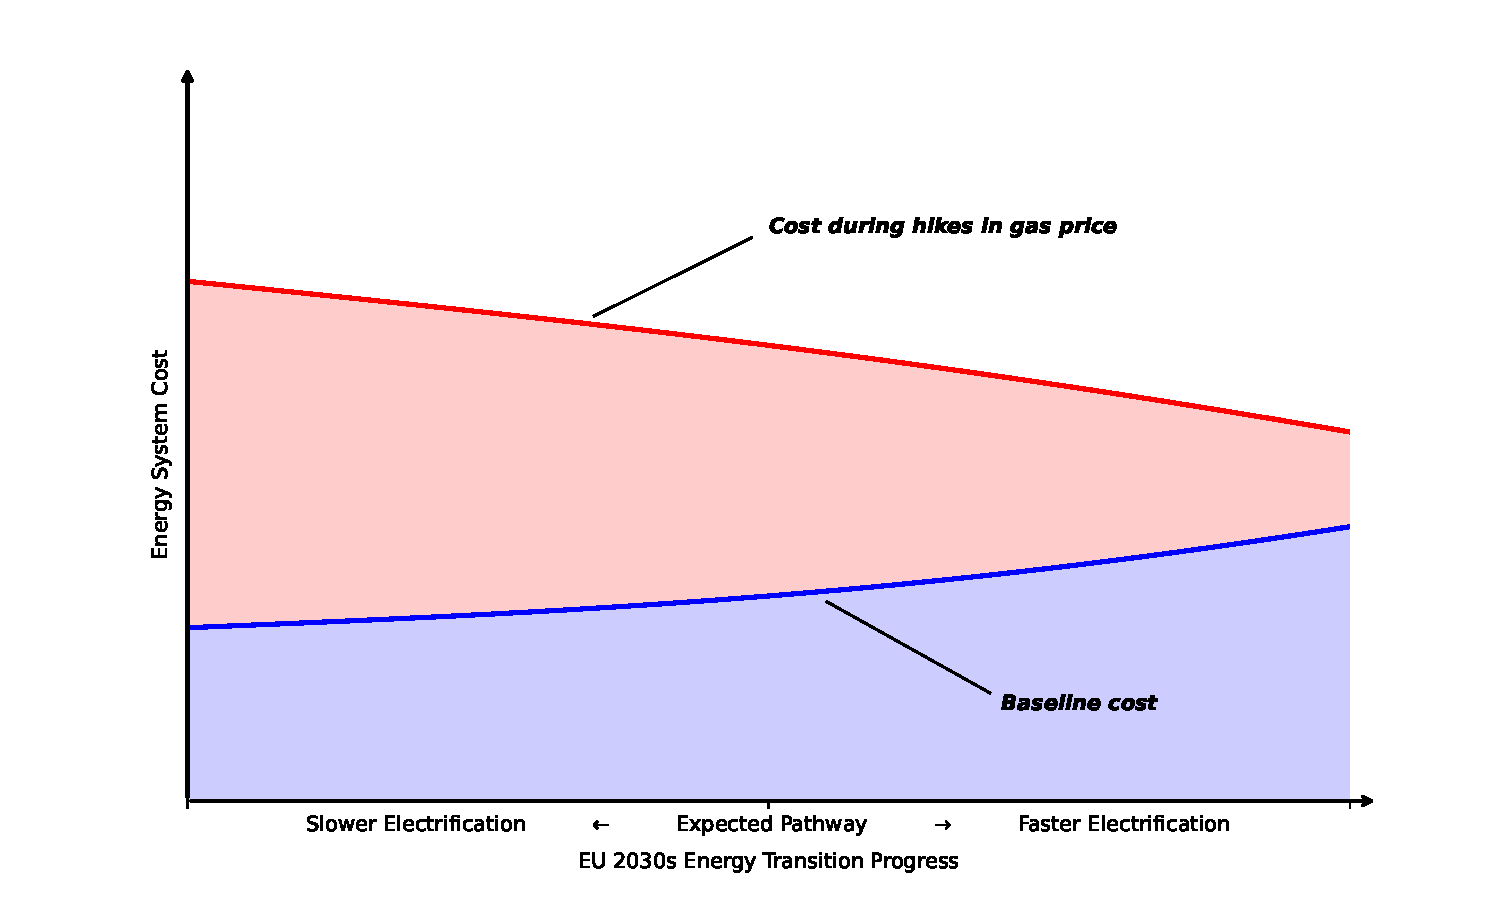
\includegraphics[width=\linewidth]{figures/gas_price_resilience_schematic}

    % Right third
    \column{0.32\textwidth}
    \centering
    
\includegraphics[width=\linewidth,height=0.22\textheight,keepaspectratio]{figures/power_sector.png}
    \vfill
    
\includegraphics[width=\linewidth,height=0.22\textheight,keepaspectratio]{figures/heating_sector.png}
    \vfill
    
\includegraphics[width=\linewidth,height=0.22\textheight,keepaspectratio]{figures/industry_sector.png}
    \vfill
    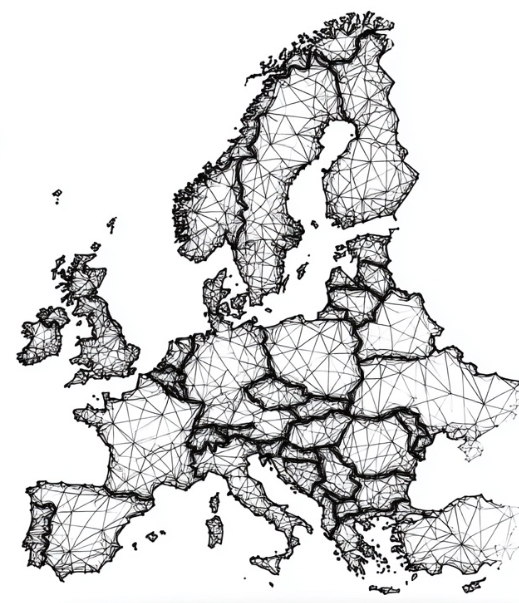
\includegraphics[width=\linewidth,height=0.22\textheight,keepaspectratio]{figures/europe.png}

  \end{columns}

\end{frame}

\begin{frame}{Extending PyPSA-Eur: Representing industrial heating by temperature band}
  \footnotesize

  \begin{columns}
    \begin{column}{0.5\textwidth}
      \footnotesize
      \begin{itemize}
        \item PyPSA-Eur represents \alert{industrial decarbonisation} by allowing a shift to alternative, low-carbon production pathways.
        \item In its current form, the model does not track the \alert{end-use of inputs}; in particular, it does not distinguish between heat use and feedstock use.
        \item The ongoing work introduces this distinction by tracking feedstock and temperature-specific heat uses, enabling the model to \alert{endogenously} simulate cost-optimal decarbonisation pathways.
      \end{itemize}
    \end{column}
    \begin{column}{0.5\textwidth}
      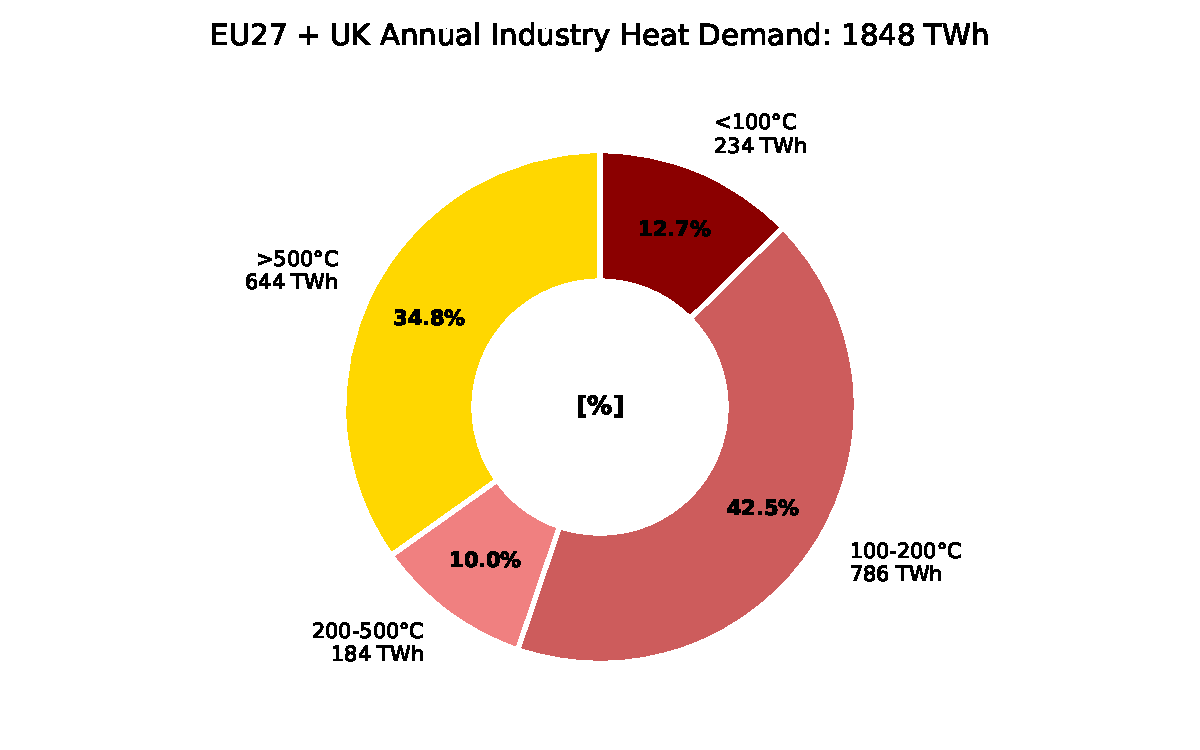
\includegraphics[width=1\textwidth]{figures/temperature_band_pie}
    \end{column}
  \end{columns}

\end{frame}

\begin{frame}
  \setbeamercolor{background canvas}{bg=red}
  \centering
  \fcolorbox{white}{tub-red}{\parbox[c][0.9\textheight][c]{\textwidth}{%
      \centering \color{white}\Large{\textbf{Thank you.}} \\ 
      \scriptsize
      \vspace{0.5cm}
      \textbf{RESILIENT} \\
      \textit{Resilient Energy System Infrastructure Layouts for Industry, E-Fuels and Network Transitions} \\
      \href{https://resilient-project.github.io}{\textcolor{white}{$\hookrightarrow$ resilient-project.github.io}} \\
      \href{https://github.com/pypsa/pypsa-eur}{\textcolor{white}{$\hookrightarrow$ github.com/pypsa/pypsa-eur}} \\
      \href{https://github.com/resilient-project/pypsa-eur-resilient}{\textcolor{white}{$\hookrightarrow$ github.com/resilient-project/pypsa-eur-resilient}} \\
      \vspace{0.5cm}
      Department of\\\textbf{Digital Transformation in Energy Systems (ENSYS)} \\
      \vspace{0.5cm}
      \textbf{Project coordination: Dr. Iegor Riepin}\\
      \href{mailto:iegor.riepin@tu-berlin.de}{\textcolor{white}{$\hookrightarrow$ iegor.riepin@tu-berlin.de}} \\
  }}
\end{frame}


% Appendix
\section{Appendix}

\begin{frame}{PyPSA-Eur: A typical model setup}
  \begin{columns}
    \begin{column}{0.5\textwidth}
      \footnotesize
      \begin{itemize}
        \setlength\itemsep{.8em}
        \item Including sectors \alert{power, heat, transport, industry, feedstock} and \alert{agriculture}
        \item Minimising \alert{total system costs} (investment and operation), including generation, transmission, storage, and power-to-X
        \item Resolving to \alert{100-200 regions}
        \item \alert{1- to 3-hourly} resolution over \alert{one year}
        \item \alert{Net-zero emission pathway} by 2050
        \item Built-in \alert{scenario manager} to handle multiple scenarios and/or \alert{stochastic optimisation}
      \end{itemize}
    \end{column}
    \begin{column}{0.5\textwidth}
      
\includegraphics[width=1\textwidth]{other/multisector_diagram}
    \end{column}
  \end{columns}

  \source{\url{https://pypsa-eur.readthedocs.io}}
\end{frame}

\begin{frame}{Exogenous demand per sector}
  \centering
  \begin{columns}
    \begin{column}{0.48\textwidth}
      \footnotesize
      \begin{figure}
        \centering
        
\includegraphics[width=1\textwidth]{exogenous_demand}
      \end{figure}
    \end{column}
    \begin{column}{0.52\textwidth}
      \footnotesize
      \begin{itemize}
        \item Demand for electricity, heat, gas, biomass, and transport is regionally and temporally resolved
        \item ICE vehicles in land transport expected to fully phase out in favour of EV by 2050
        \item Demand for methanol and hydrocarbons, including kerosene primarily driven by shipping, aviation, and industry sector (not spatially resolved)
        \item Unabatable process emissions from industry sector, e.g. cement, also considered
        \item \ce{CO2} sequestration cost assumed at \euro{15}/t\ce{CO2} (mid-range estimate)
      \end{itemize}
    \end{column}
  \end{columns}
  \source{Preprint Xiong, Brown, Riepin (2025):\\\url{https://doi.org/10.48550/arXiv.2507.01860}}
\end{frame}

\begin{frame}{Electricity vs. hydrogen network expansion}
  \centering
  
\includegraphics[width=0.9\textwidth]{other/neumann_hydrogen_paper}
  \\
  \footnotesize
  $\rightarrow$ Hydrogen grid \alert{reduces system costs}, but \alert{electricity grid expansion is more attractive.} \\

  \source{Neumann, Zeyen, Victoria, Brown:\\\url{https://doi.org/10.1016/j.joule.2023.06.016}}
\end{frame}


\begin{frame}{Why H$_2$? Most H$_2$ is used for derivative fuels and chemicals}
  
  
\includegraphics[width=1.2\textwidth, trim=0cm 6.6cm 0cm 6.6cm, clip]{other/hydrogen_balance.pdf}

  \footnotesize

  Mostly \alert{green electrolytic hydrogen supply}. \alert{Few direct uses of hydrogen} in the energy system, but it is used to synthesise other fuels and chemicals:

  \begin{multicols}{2}
    \begin{itemize}
      \item ammonia for fertilizers
      \item direct reduced iron for steelmaking
      \item shipping and aviation fuels
      \item precursor to high-value chemicals
      \item backup heat and power supply
      \item some heavy duty land transport
    \end{itemize}
  \end{multicols}

  \source{Neumann, Zeyen, Victoria, Brown (2023): \\\url{https://doi.org/10.1016/j.joule.2023.06.016}}
\end{frame}

\begin{frame}{Carbon management: Capture, use, transport and sequestration}
  
  \begin{center}
    
\includegraphics[height=0.73\textheight]{other/carbon_networks_cost_bar}
    
\includegraphics[height=0.71\textheight]{other/carbon_networks_balance_bar_carbon}

    \vspace{-0.25cm}
    \footnotesize
    \begin{itemize}
      \item \alert{CCS} for process emissions (for instance, in cement industry)
      \item \alert{CCU} for e-synfuels and e-chemicals (in particular, shipping, aviation, plastics)
      \item \alert{CDR} for unabatable and negative emissions (to offset imperfect capture rates)
    \end{itemize}

  \end{center}

  \source{Hofmann, Tries, Neumann, Zeyen, Brown (2024): \\\url{https://www.nature.com/articles/s41560-025-01752-6}}

\end{frame}


\begin{frame}{Electricity high-voltage grid based on OpenStreetMap (OSM)}

  \begin{columns}
    \begin{column}{0.64\textwidth}
      \footnotesize
      \begin{itemize}
        \setlength\itemsep{.8em}
        \item Dataset contains a topologically connected representation of the European high-voltage grid (220 kV to 750 kV) constructed using OpenStreetMap data
        \item Heuristic cleaning process was used to for lines and links where electrical parameters are incomplete, missing, or ambiguous
        \item Close substations within a radius of 500 m are aggregated to single buses
        \item Unique transformers are added for each voltage pair in a substation
        \item AC lines mapped using pandapower's standard line type library. In default version, nominal capacity is set to 70 \% of the technical capacity to account for n-1 security approximation
        \item Includes all 38 European HVDC connections with their nominal rating that are commissioned as of 2024
      \end{itemize}
    \end{column}
    \begin{column}{0.36\textwidth}
      
\includegraphics[width=1\textwidth]{osm_map}
    \end{column}
  \end{columns}
  \source{Xiong, Fioriti, Neumann, Riepin, Brown (2025):\\\url{https://www.nature.com/articles/s41597-025-04550-7}}
  
  
\end{frame}

\end{document}